\subsection*{Solution 10}

\begin{itemize}
\item[(a)]

\begin{itemize}

\item[(i)]

The function $f(z)$ has two simple poles at $z=1$ and $z=5$.

\item[(ii)]

A sketch of the annulus is shown below:

%
%	Sketches for Q10(a)(i)

%
%	The annulus {z: 1 < |z-2| < 3}
%
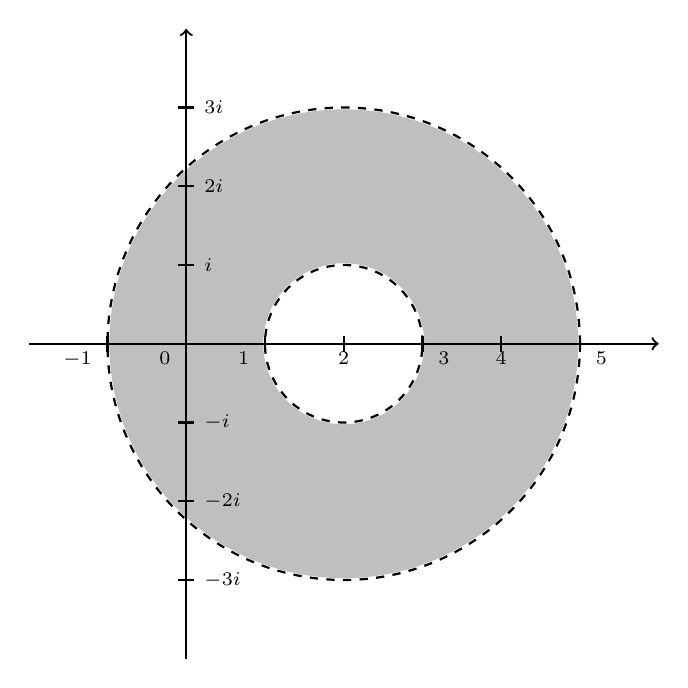
\begin{tikzpicture}
	% shading - must be drawn before the rest!
	\filldraw[even odd rule,color=lightgray] (2,0) circle(2.97) (2,0) circle(1.03);
	% grid for draft only
	%%\draw [help lines] (-2,-4) grid (6,4);
	% the X-axis
	\draw[->,thick] (-2,0)--(6,0);
	\foreach \x in {-1, 0, 1} {
		\draw[thick] (\x,-0.1) -- (\x,0.1) node[below left=2pt] {\scriptsize $\x$};
	}
	\foreach \x in {2, 4} {
		\draw[thick] (\x,-0.1) -- (\x,0.1) node[below=2pt] {\scriptsize $\x$};
	}
	\foreach \x in {3, 5} {
		\draw[thick] (\x,-0.1) -- (\x,0.1) node[below right=2pt] {\scriptsize $\x$};
	}
	% the Y-axis
	\draw[->,thick] (0,-4)--(0,4);
	\foreach \y in {2, 3} {
		\draw[thick] (-0.1,-\y) -- ( 0.1,-\y) node[right] {\scriptsize $-\y i$};
		\draw[thick] (-0.1, \y) -- ( 0.1, \y) node[right] {\scriptsize $ \y i$};
	}
	\draw[thick] (-0.1,-1) -- (0.1,-1) node[right] {\scriptsize $-i$};
	\draw[thick] (-0.1, 1) -- (0.1, 1) node[right] {\scriptsize $ i$};
	% inner circle border
	\draw[thick,style=dashed] (2,0) circle (1);
	% outer circle border
	\draw[thick,style=dashed] (2,0) circle (3);
\end{tikzpicture}



\todo
\end{itemize}

\item[(b)]

\begin{itemize}
\item[(i)]
\todo
\item[(ii)]
\todo
\end{itemize}

\end{itemize}

